\section{Verifying Properties of DSLTrans Transformations}
\label{sec:verif_dsltrans_props}

% As we have mentioned in section~\ref{sec:dsltrans}, all DSLTrans transformations
% are, by construction, \emph{terminating} and
% \emph{confluent}~\cite{DBLP:conf/sle/BarrocaLAFS10}. We have also abstractly
% shown in~\cite{Lucio:10} how to build a symbolic execution such that
% properties of DSLTrans transformations can be proved. We formally prove
% in~\cite{Lucio:10}, proposition 2, that such a symbolic execution is always
% finite. With our current work we aim at producing a tool that can prove or
% disprove such properties efficiently. 

The algorithm presented in \cref{sec:building_pcs} will produce all possible
path conditions for a given DSLTrans transformation. This section will detail
our second contribution: a method to prove properties on the transformation by
examining the path conditions generated for it. We then rely on the abstraction
relation presented in~\cref{def:abstraction_pc_ex} to extrapolate the proof
result to all of the transformation's executions.

The properties we are interested in have an implication form. Similarly to rules and path conditions, properties are largely composed of two patterns. They represent the following statement: whenever this pattern is found in the input model, then
this other pattern must be found in the output model, possibly including traceability constraints.

The property proving algorithm is relatively simple. The match part of a path condition
includes a representation of all the elements and relations ``touched'' in the input model of a set of transformation executions. Likewise, the property's pre-condition pattern represents the prerequisite for the property. Thus, the
property proving algorithm will attempt to find the property's pre-condition pattern in the path condition's match graph. If not found, then the property will not be validated on this path condition, as the prerequisites do not exist.

Whenever the property's pre-condition pattern is found, the property's
post-condition pattern is searched for in the path condition. If
also found, then the rule execution(s) defined by that path condition will produce
the required elements for that property and the property will hold. If not
found, then the necessary elements will not be produced and the property check
will fail for that path condition.

Path conditions for a transformation are checked to understand whether the property of interest holds on all of them. If it does, then by making use of the abstraction relation in \cref{sec:abstraction_relation} between path conditions and transformation executions, we can deduce that the property then holds for all transformation executions. If not, we deduce the property does not hold for at least one transformation execution. Later in this section we will develop a formal argument for why this is true.

\subsection{Structure of a Property}
We will now elaborate on the structures and the relations required for the property proving algorithm. Let us start by precisely defining what a property of a transformation is. 


\begin{definition}{Property of a Transformation\\}
\label{def:trans_prop}
\CatchFileBetweenTags{\propertydef}{text/definitions}{propertydef}{\propertydef}
\end{definition}

%Property proving then becomes relatively simple. The path condition match graph
%represents the elements which define that path condition. Likewise, the property
%pre-condition pattern represents the prerequisite for the property. Thus,
%property proving algorithm will attempt to isomorphically find the property's
%pre-condition pattern in the path condition's match graph. If not found, then the
%property will not be validated on this path condition, as the prerequisites do
%not exist.

%If the property's pre-condition pattern is found, then the property's
%post-condition pattern is isomorphically searched for in the path condition. If
%it is found, then the rule execution defined by that path condition will produce
%the required elements for that property and the property will hold. If not
%found, then the necessary elements will not be produced and the property check
%will fail.

%In this way, all path conditions are checked to see if the property specified is
%applicable to that execution, and then if the execution satisfies that property.
%Therefore, properties can be verified for all possible executions of a
%ransformation using the abstraction relation.

%These constraints are expressed as graph patterns on the
%\emph{match graph} and \emph{apply graph} of DSLTrans transformation rules.

% \levi{Needs revision}
% In~\cite{Narayanan:07} Narayanan and Karsai describe the nature of these model
% syntax relation properties, which they call called \emph{structural
% correspondence rules} in their work. As the authors claim, ``\emph{given the
% correspondence conditions are specified in terms of simple queries on the model
% around previously chosen context (metamodel) nodes, we expect that they will be
% easier to specify, and thus more reliable than the transformation itself}''.

In \cref{def:trans_prop}, pre-conditions use the same pattern language as the match graph in
DSLTrans rules, allowing the possibility of including several instances of
the same metamodel element as well as indirect links in the property. Indirect links in properties have
the same meaning as in the rule match graph -- they
involve patterns over the transitive closure of containment links in pre-condition graphs.

Post-conditions also use the same pattern language as the
apply graphs of DSLTrans transformation rules, with the additional
possibility of expressing indirect links in post-conditions. Traceability links can
also be used in properties to impose traceability relations between pre-condition
and post-condition elements.

Note that \cref{def:trans_prop} includes a condition stating a surjective typed graph homomorphism needs to exist between the match part of at least one of the transformation's path condition, and the pre-condition of the property of interest. This condition makes sure that the property's pre-condition can be found at least in one execution of the transformation abstracted (the mathematical argument for this fact is given in the proof of \cref{prop:proof_validity}). This condition makes the checking the validity of a property in the transformation meaningful. If this condition would not be true then it could be that the input pattern required by the property would never be fully matched during transformation execution, making such a property not relevant\footnote{In~\cite{DBLP:conf/sle/BarrocaLAFS10} we have referred to these properties \emph{non-provable}. In the work presented here we explicitely disallow the construction of this class of properties.} for the transformation at hand.

% This last condition explicitly restricts the approach to properties which pre-condition can be \emph{found} in the match part of a path condition of the considered transformation. 

% Note that by \emph{found}, we mean that these pre-conditions need to be isomorphically matched on at least one graph resulting from overlapping elements of the same type (but belonging to different rules) in the match part of at least one path condition of the transformation. This overlapping between rules allows taking into account the fact that different rules in a path condition may have match elements of the same type that can potentially match (overlap) over the same class instance in an input model, when a transformation execution is built. This potential overlapping of rules in the path condition is modeled by the surjection in definition~\ref{def:trans_prop} between (a subgraph of) the path condition and the property.


%This would required considering more than one copy of the same rule in the same path condition.  
% \levi{unclear}
% In our symbolic execution algorithm, path conditions are built relying only on
% the rules of the DSLTrans transformation we are analysing. These path conditions
% are built to symbolically represent all possible executions of that DSLTrans
% transformation. Thus, if our prover algorithm replies \emph{yes}, then the
% precondition-postcondition implication expressed in the property will hold for
% all executions of the DSLTrans transformation under analysis. On the other hand,
% if the prover replies \emph{no}, then that will mean that there exists at least
% one exception to the implication in the property. In other words, there exists
% at least one model in which the precondition of the property holds, but the
% postcondition does not. A counter-example can be provided in this case,
% consisting of the set of rules that, when executed, lead to the property being
% violated.

%In figures~\ref{fig:dsltrans_prop1} and~\ref{fig:dsltrans_prop2} we present two
%properties we wish to prove or disprove regarding all executions of the
%transformation presented in \cref{fig:dsltransformation}.\levi{remove figures of properties} The property in
%\cref{fig:dsltrans_prop1} represents the statement ``\emph{a model which includes a
%police station that has both male and female officers will be
%transformed into a model where the male officer will exist in the male set
%and the female officer will exist in the female set}''. This is something
%we expect will always hold in our transformation. The property in
%\cref{fig:dsltrans_prop2} represents the statement ``\emph{any model which includes a
%female officer will be transformed into a model where that female officer will
%always supervise another female officer}'', which is something that we expect
%will hold for our transformation sometimes, but not always.
%
%\begin{figure}[htb]
%        \centering
%        \begin{subfigure}[b]{0.45\textwidth}
%                \centering
%                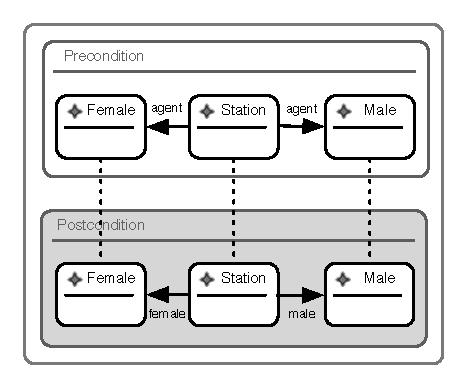
\includegraphics[width=1\textwidth]{./figures/policestation_dsltrans/satisfied.pdf}
%                \caption{Property 1 -- Expected to hold}
%                \label{fig:dsltrans_prop1}
%        \end{subfigure}%
%        ~~
%        \begin{subfigure}[b]{0.45\textwidth}
%                \centering
%                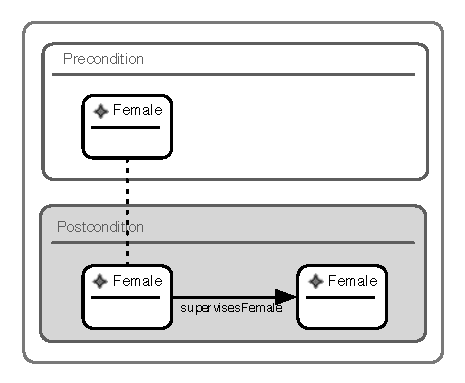
\includegraphics[width=1\textwidth]{./figures/policestation_dsltrans/unsatisfied.pdf}
%                \caption{Property 2 -- Not expected to hold}
%                \label{fig:dsltrans_prop2}
%        \end{subfigure}%
%        \caption{ Properties to be proved on the Police Station transformation}
%        \label{fig:properties}
%\end{figure}

\subsection{Satisfaction of a Property}
\label{sec:prop_satisfaction}

Let us now detail how a transformation execution is said to satisfy a property. Due to the common structure between properties and transformation executions, this satisfaction is based on whether the property can be isomorphically found in the transformation execution.

\begin{definition}{Satisfaction of a Property by an Execution of a Transformation\\}
\label{def:sat_prop_ex}
\CatchFileBetweenTags{\satpropexe}{text/definitions}{satpropexe}{\satpropexe}
\end{definition}

\Cref{def:sat_prop_ex} states that, every time a graph that is isomorphic to the property's pre-condition is found in (the containment transitive closure of) the input model of the transformation's execution, a graph that is isomorphic to the complete property needs to be found in (the containment transitive closure of) the transformation execution. Note that the last part of the proposition in \cref{def:sat_prop_ex} ensures that the graph that is isomorphic to the property's pre-condition and the graph that is isomorphic to the complete property overlap on their pre-condition parts.

% resulting from the input pattern of $ex$ identified as pre-condition by $f$. Generally speaking, whenever the property's pre-condition is isomorphically found as a pattern of the input model of a execution, the property's post-condition must also be isomorphically found in the output generated from that input pattern. Note that, because a property may contain traceability links between the pre- and post-condition elements, it is necessary to check that those traceability links are also present in the execution. Because of this, the $g$ homomorphism in definition~\ref{def:sat_prop_ex} that checks the property's post-condition is such that it considers the same match pattern identified by the $f$ homomorphism when the pre-condition is checked.

\Cref{fig:prop_execution_without_traceability} demonstrates how a property holds on a transformation execution. Note that the lack of traceability links in the property means no element creation dependencies have been specified. In contrast, the traceability links in the property in \cref{fig:prop_execution_with_traceability} specify that the 'x:X' element must have been created from the 'b:B' element in the transformation execution. This is not the case (as highlighted by the dashed red circle), and therefore the property does not hold on the transformation execution.

\begin{figure}[htb]
        \centering
        \begin{subfigure}[b]{0.40\textwidth}
                \centering
                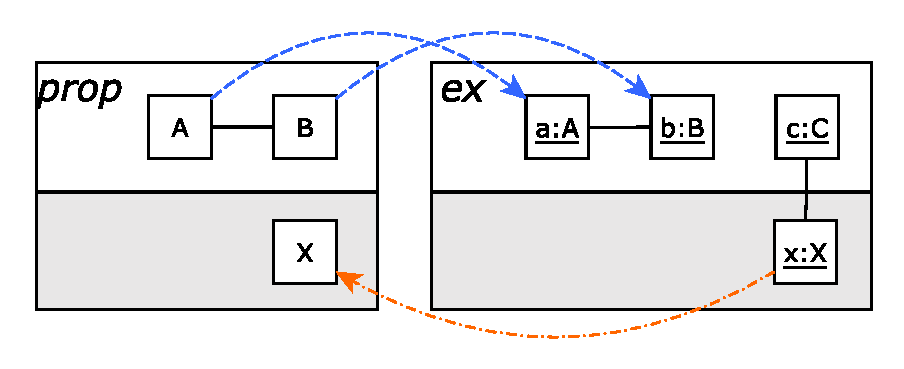
\includegraphics[width=1\textwidth]{./figures/property_proving/prop_execution_without_traceability.pdf}
                \caption{Property holds}
                \label{fig:prop_execution_without_traceability}
        \end{subfigure}%
        \\
        \begin{subfigure}[b]{0.40\textwidth}
                \centering
                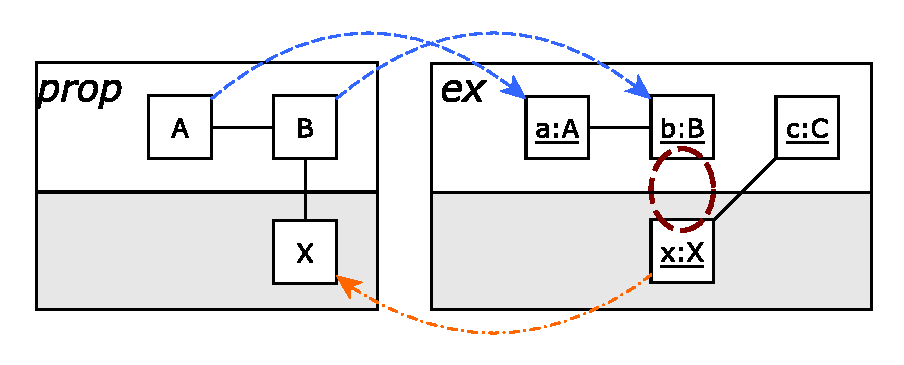
\includegraphics[width=1\textwidth]{./figures/property_proving/prop_execution_with_traceability.pdf}
                \caption{Property does not hold}
                \label{fig:prop_execution_with_traceability}
        \end{subfigure}%
        \caption{Matching property to a transformation execution}
        \label{fig:prop_execution}
\end{figure}

% \cref{def:sat_prop_pc} is similar to that of property satisfaction for a transformation execution, but for path conditions. Again, the property is isomorphically matched onto the respective graphs in the path condition.
% 
% Properties are proved on each path condition created by the path condition generation algorithm. Each path condition is examined to determine whether the pre-condition graph of the property can be isomorphically matched onto the match graph of the path condition, as in \cref{def:sat_prop_pc}. If this match cannot be performed, then the pre-condition does not hold for this path condition and this path condition will not be checked for this property.
% 
% If the pre-condition can be isomorphically matched to the match graph of the path condition, then we check if the entire
% property can be isomorphically matched to the path condition. Again, this is described in \cref{def:sat_prop_pc}. If this matching cannot be performed, then the property does not hold. The path condition itself then serves as a
% counter-example for the transformation property. The path condition also contains information on which rules were executed in the counter-example to permit further examination.
% 
% This property-checking can be done relatively quickly with efficient graph-matching techniques. \cref{sec:implementation} will briefly describe implementation and optimization details, while \cref{sec:experiments} presents two property-proving experiments.

Due to the fact an infinite amount of transformation executions exists, proving the property directly on the set of transformation executions is not possible. We thus rely on the finite set of path conditions to prove properties about the set of all transformation execution. Let us then define what it means for a property to hold on, or be satisfied by, a path condition.  

\begin{definition}{Satisfaction of a Property by a Path Condition\\}
\label{def:sat_prop_pc}
\CatchFileBetweenTags{\satproppc}{text/definitions}{satproppc}{\satproppc}
\end{definition}

The principle behind the satisfaction relation in \cref{def:sat_prop_pc} is the same as the one behind the satisfaction relation between a property and an execution of a transformation in \cref{def:sat_prop_ex}: whenever the property's pre-condition is found in the path condition then so is the complete property. Also, those two graphs found in the path condition share the property's pre-condition part. This last condition enforces that the pre- and post-conditions of the property are correctly linked by symbolic traceability links in the path condition.

Note that, despite their semantic similarity, the relations are expressed differently in \cref{def:sat_prop_ex} and \cref{def:sat_prop_pc}. In \cref{def:sat_prop_ex} -- \emph{satisfaction of a property by an execution of a transformation}, typed graph injective homomorphisms are defined from the property into the execution. However, in \cref{def:sat_prop_pc} the direction of the typed graph surjective homomorphisms is from the path condition into the property. This can be explained by the fact, mentioned previously in this text, that different rules in a path condition may have elements that match over the same concrete instances of a transformation's input model. As such, we need to consider the case where match elements of a path condition, originating from different rules, overlap. 

\begin{figure}[htb]
 \centering
                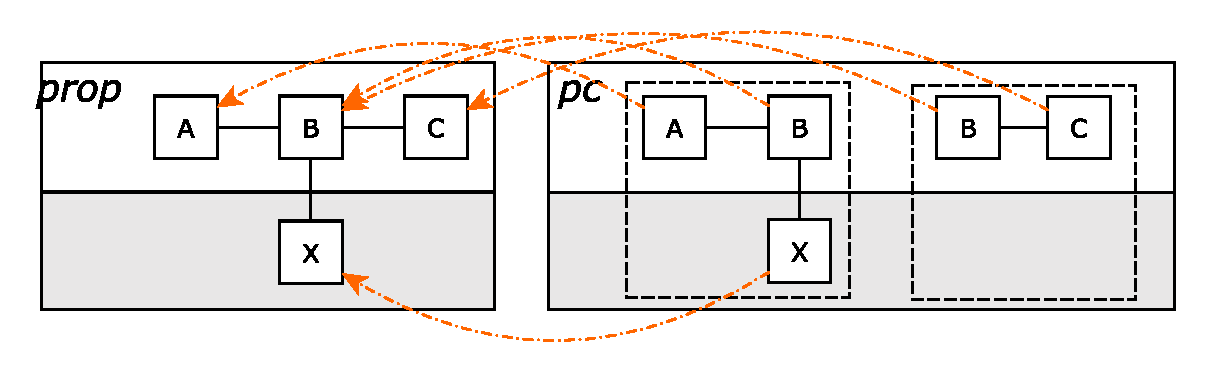
\includegraphics[width=0.44\textwidth]{./figures/property_proving/prop_pc.pdf}
                \caption{Property satisfied by a path condition}
                \label{fig:prop_pc}
\end{figure}

This overlapping is modeled by the surjective typed graph homomorphisms of \cref{def:sat_prop_pc} having the property as co-domain. The surjections allow ``forgetting'' that two match elements of the path condition belong to different rules. Note however that these surjections are special, as two elements belonging to the same copy of a rule have to be mapped injectively onto the property. This situation is depicted in \cref{fig:prop_pc}. Note that element $B$ is successfully matched even though it appears in two different rules in the path condition. 



\subsection{Expressiveness of the Property Language}
\label{subsec:expressiveness_prop}

As a result of taking rule combination (\cref{sec:building_pcs}) and overlap (\cref{sec:prop_satisfaction}) into consideration, our technique allows proving properties of transformation executions that are matched and built by multiple rules. This is the main goal of our work, as the properties we are interested in regard all possible interactions of rules in a DSLTrans transformation. However, an expressiveness limitation of the property language exists: we cannot prove properties having pre-conditions that can be found by executing the exact same rule more than once. This is natural, as by definition our abstraction only considers one exemplar of each rule per path condition having the exact same type for each match element. 

In order to illustrate this limitation, consider a transformation having one single rule that matches an element of type A and that produces an element of type X. Our technique will create a path condition as seen in \cref{fig:unprovable_pc}, abstracting over the number of times this rule has executed. According to the definition of satisfaction of a property by a path condition in \cref{def:sat_prop_pc}, the property in \cref{fig:unprovable_prop} does not hold on the path condition in \cref{fig:unprovable_pc}, although intuitively it should.

\begin{figure}[htb]
        \centering
        \begin{subfigure}[b]{0.144\textwidth}
                \centering
                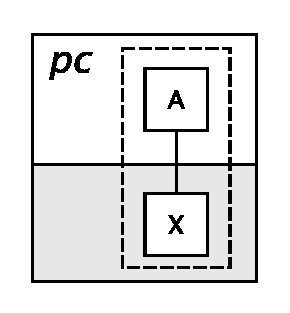
\includegraphics[width=1\textwidth]{./figures/property_proving/unprovable_rule.pdf}
                \caption{Path condition created from a rule}
                \label{fig:unprovable_pc}
        \end{subfigure}%
        ~~
        \begin{subfigure}[b]{0.20\textwidth}
                \centering
                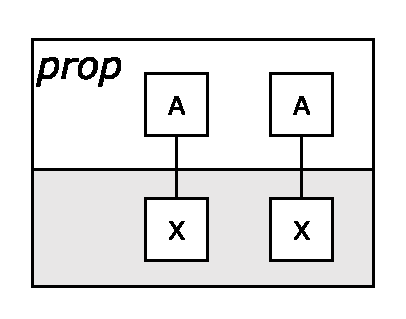
\includegraphics[width=1\textwidth]{./figures/property_proving/unprovable_prop.pdf}
                \caption{Property with multiple instances of rule elements}
                \label{fig:unprovable_prop}
        \end{subfigure}%
        \caption{Example of unprovable property}
        \label{fig:unprovable_property}
\end{figure}

Although this might be seen as a limitation of our technique, our case studies thus far indicate that very interesting properties exist that exclusively regard interactions between different rules. Nonetheless, our technique could be extended in order to consider more than one exemplar of the same rule per path condition. In fact, theoretically we already consider more than one exemplar of each rule when we treat polymorphism during path condition generation (see \cref{def:path_cond_gen}). However, in this case all expanded rules for a rule $rl$ are considered to be different as they differ by at least the type of one match element. Although this extension seems to fit relatively simply in our current theory, additional steps would need to be taken to understand which rules would be interesting to replicate to prove a particular property, and how many exemplars of each rule should be considered. In operational terms the number of replicas to consider of each rule is very important, given the exponential complexity of our path condition generation and property proof algorithms. Another possibility to tackle this issue would be to investigate and implement a more powerful satisfaction relation between path conditions and properties than the one we now present in \cref{def:sat_prop_pc}.
%Note however that the homomorphisms are injective when two elements belong to the same rule.\levi{explain this better}

% Given these definitions, we see that as all transformation executions are represented by path conditions, proving properties on the path conditions allows us to conclude property validity on all transformation executions.


